% concatenated from main.tex
\documentclass[journal]{IEEEtran}

% *** CITATION PACKAGES ***
\usepackage{cite}

%Matlab2tikz related
  \usepackage{pgfplots}
  \pgfplotsset{compat=newest}
  %% the following commands are needed for some matlab2tikz features
  \usetikzlibrary{plotmarks}
  \usetikzlibrary{arrows.meta}
  \usepgfplotslibrary{patchplots}
  \usepackage{grffile}

% Tikz
\usepackage{tikz}
\usetikzlibrary{arrows.meta,positioning,fit,calc}


% *** GRAPHICS RELATED PACKAGES ***
\usepackage{graphicx}
\usepackage{xcolor}
\usepackage{tikz}
\usetikzlibrary{shapes,arrows}
%\usepackage{subcaption}
\usepackage[table]{xcolor}
\usepackage{booktabs}
\usepackage{balance}

\usepackage[caption=false,font=footnotesize]{subfig} % IEEEtran-friendly subfig
% If you compile with pdflatex and have EPS inputs:
% \usepackage{epstopdf} % converts .eps on the fly

% *** MATH PACKAGES ***
\usepackage{amsmath,amssymb,amsfonts, amsthm}

% *** ALGORITHM PACKAGES ***
\usepackage[ruled,vlined]{algorithm2e}
\usepackage{enumitem}
\newtheorem{remark}{Remark}
\newtheorem{lemma}{Lemma}
\newtheorem{theorem}{Theorem}
\newtheorem{corollary}{Corollary}
\newtheorem{proposition}{Proposition}
% *** For code/listings (if needed) ***
\usepackage{listings}
\lstset{
   basicstyle=\footnotesize\ttfamily,
   columns=fullflexible,
   breaklines=true,
   captionpos=b,
   frame=single,
   numbers=left,
   numberstyle=\tiny,
   keywordstyle=\color{blue},
   commentstyle=\color{teal},
   stringstyle=\color{red},
}


\begin{document}
\title{On the Structure of the Optimal Detector for Sub-THz Multi-Hop Relays with Unknown Prior: Over-the-Air Diffusion
}

\author{Ozgur Ercetin, and Mohaned Chraiti%
\thanks{The authors are with the Faculty of Engineering and Natural Sciences, Sabanci University, Istanbul, Turkey (e-mail: \{oercetin, mohaned.chraiti\}@sabanciuniv.edu).}%
}


\maketitle

\begin{abstract}
Amplify-and-forward (AF) relaying is an viable strategy to extend the coverage of sub-terahertz (sub-THz) links, but inevitably propagates noise, leading to cumulative degradation across multiple hops. At the receiver, optimal decoding is derisible, yet challenging under non-Gaussian input distributions (video, voice, etc), for which neither the Minimum Mean Square Error (MMSE) estimator nor the mutual information admits a closed form. A further open question is whether or not the knowledge of Channel State Information (CSI) and noise statistics at the intermediate relays are necessary for optimal detection. Aiming for optimal decoder, this paper introduces a new framework that interprets the AF relay chain as a variance-preserving diffusion process and employs denoising diffusion implicit models (DDIMs) for signal recovery. We show that each AF hop is mathematically equivalent to a diffusion step with hop-dependent attenuation and noise injection. Consequently, the entire multi-hop chain collapses to an equivalent Gaussian channel fully described by only three real scalars per block: the cumulative complex gain and the effective noise variance. At the receiver, these end-to-end sufficient statistics define a matched reverse schedule that guides the DDIM-based denoiser, enabling near-optimal Bayesian decoding without per-hop CSI. We establish the information-theoretic foundation of this equivalence, proving that decoding performance depends solely on the final effective Signal-to-Noise-Ratio (SNR), regardless of intermediate noise/channel allocation or prior distribution. Simulations under AWGN and Rician fading confirm that the proposed AF–DDIM decoder significantly reduces mean-squared error, symbol error rate, and bit error rate, particularly at moderate SNRs and for higher-order constellations.



 %Amplify-and-forward (AF) relays is deemed to be effcinet way to extend coverage of sub-terHertz (sub-THz), yet unavoidably propagate noise, causing cumulative degradation across multiple hops. At the receiver side, the best case snacrio is to opt for optimal decoder, which deammed to be chnallenging espcially knwnig that the trasnmitted data (prior) is not Guassian and hence the MMSE nor the mutual information has tracable format. In the chase of the optimal decider, other question may raise including whether the knolwfge pf intermidate channel coffcienc and noise staticts have an impact on the optimilzaty of the devoder. This paper introduces a framework that interprets the AF relay chain as a deterministic diffusion process and leverages denoising diffusion implicit models (DDIMs) for signal recovery. Each relay hop is shown to be equivalent to a diffusion step with hop-dependent attenuation and noise injection, allowing sufficient statistics to be propagated end-to-end with only three real scalars per block. At the receiver, these statistics define a matched reverse schedule that guides the DDIM-based denoiser, yielding an optimla decoder with channel-compensated reconstruction without requiring per-hop channel state indicator (CSI). We prove through information theory and sttics that thi sprocess lead to optimal deciodeer strcture. Numerical experiments under additive white Gaussian noise (AWGN) and Rician fading demonstrate that our approach significantly reduces mean-squared error (MSE), symbol error rate (SER), and bit error rate (BER), particularly at moderate SNRs and for higher-order constellations. 



%Sub-terahertz (sub-THz) communication promises unprecedented data rates but suffers from severe path loss and molecular absorption, limiting single-hop transmission to only a few meters. Amplify-and-forward (AF) relays extend coverage, yet unavoidably propagate noise, causing cumulative degradation across multiple hops. This paper introduces a framework that interprets the AF relay chain as a deterministic diffusion process and leverages denoising diffusion implicit models (DDIMs) for signal recovery. Each relay hop is shown to be equivalent to a diffusion step with hop-dependent attenuation and noise injection, allowing sufficient statistics to be propagated end-to-end with only three real scalars per block. At the receiver, these statistics define a matched reverse schedule that guides the DDIM-based denoiser, yielding a channel-compensated reconstruction without requiring per-hop channel state indicator (CSI). Numerical experiments under additive white Gaussian noise (AWGN) and Rician fading demonstrate that our approach significantly reduces mean-squared error (MSE), symbol error rate (SER), and bit error rate (BER), particularly at moderate SNRs and for higher-order constellations. 
\end{abstract}

\begin{IEEEkeywords}
Denoising diffusion probabilistic models, amplify-and-forward relaying, sub-terahertz communication, multi-hop networks, generative signal recovery, low-overhead detection.
\end{IEEEkeywords}



\section{Introduction}
Sub-terahertz (sub-THz) communication, operating in the 0.1--1\,THz spectrum, promises ultra-high data rates necessary for future wireless systems~\cite{rappaport2019wireless,koenig2013wireless}. Yet, the pronounced free-space path loss at these frequencies confines viable transmission to short-range scenarios. In indoor environments—comprising corridors, partitions, and reflective surfaces—such attenuation is compounded by complex multipath effects~\cite{goldsmith2005wireless}. To counteract this, fixed-gain amplify-and-forward (AF) relays have emerged as a pragmatic mechanism for extending link coverage across segmented indoor topologies.

While AF relays offer signal amplification, they inherently propagate additive noise, which accumulates across hops and degrades the end-to-end signal integrity. Passive alternatives, such as reconfigurable intelligent surfaces, while immune to noise amplification, lack the power gain required to counterbalance sub-THz path loss. Consequently, fixed-gain AF remains an indispensable architecture in such high-frequency networks, despite its deleterious noise compounding.

At the receiver, optimal detection is fundamentally achieved by the Bayes-optimal minimum mean-square error (MMSE) estimator. However, in AF multi-hop relaying, this detector requires evaluating the posterior distribution of the source given the noisy observations, which entails marginalization over the input prior. In practical scenarios—such as multimedia transmissions of video or voice—the source distribution is generally non-Gaussian, stochastic, and time-varying. Assuming Gaussian priors is therefore unrealistic, and renders closed-form MMSE estimators or mutual information expressions analytically intractable and computationally prohibitive. Consequently, existing works often resort to suboptimal linear MMSE filters, which presume stationary Gaussian noise and fixed end-to-end channel gains, resulting in significant performance loss under realistic AF chains. A further question is whether knowledge of intermediate-hop channel state information (CSI) or noise statistics could improve detection. As we show later, such intermediate information is redundant once the end-to-end sufficient statistics are known.

Motivated by these limitations, this work introduces a new perspective: multi-hop AF relaying can be interpreted as a physical realization of a forward variance-preserving diffusion process \cite{ho2020denoising,sohl2015deep}. Each hop injects Gaussian noise and attenuation, exactly mirroring a diffusion step. At the receiver, the reverse denoising process can be carried out using a schedule derived solely from end-to-end sufficient statistics, without relying on per-hop CSI or processing at intermediate relays. This interpretation aligns with practical constraints, particularly in fixed-gain deployments \cite{bhardwaj2022fixed}, while enabling a fundamentally new class of receiver designs.

Our work advances sub-THz relay networks through:
\begin{itemize}
    \item {Over-the-Air Diffusion:} We establish a direct correspondence between multi-hop AF relaying and a deterministic diffusion forward process, where each hop injects Gaussian noise and attenuation. This interpretation provides a physically grounded generative channel model.

    \item {End-to-End Sufficient Statistics:} We prove that the AF chain collapses into two statistics—a composite complex gain and an effective noise variance—that are information-equivalent to full CSI. Only three real scalars per block are required for SISO, or per eigenmode after whitening in MIMO systems. This equivalence also allows training and reverse denoising with arbitrary numbers of hops, provided the effective SNR is preserved. 

    \item {Channel-Matched Diffusion Scheduling:} We derive a per-sample noise schedule from the equivalent SNR, ensuring that the reverse denoising process is aligned with the realized propagation conditions, without requiring per-hop CSI at the receiver.

    \item {Low-Overhead Implementation:} We quantify the signaling overhead of sufficient statistics, showing that even with conservative quantization, the data utilization exceeds $95\%$ for modest block sizes. This validates our approach as a practical solution for high-throughput sub-THz relay networks.
\end{itemize}



% This paper is organized as follows. Section~\ref{sec:related_work} reviews prior work in sub-THz relaying and machine-learning-based signal recovery. Section~\ref{sec:system_model} introduces the physical and statistical model for multi-hop AF propagation. Section~\ref{Sec:DDPM} formulates the relay chain as a DDPM and defines the reverse generative process. Section~\ref{sec:variational_reverse} presents a variational inference approach to score modeling. Section~\ref{sec:topology_schedule} aligns the diffusion schedule with system topology. Section~\ref{sec:implementation} details the training method and implementation. Section~\ref{sec:results} reports simulation results comparing our approach with MMSE baselines. Section~\ref{sec:conclusion} concludes and outlines future directions.

\section{Related Work}
\label{sec:related_work}

\subsection{Sub–THz Links and Multi–Hop Relaying}
Sub–THz communication promises ultra–high data rates but faces severe path loss, atmospheric absorption, and hardware constraints, which limit link budget and range \cite{rappaport2019wireless,koenig2013wireless}. Multi–hop relaying has therefore been widely investigated as a range–extension mechanism \cite{goldsmith2005wireless,boulogeorgos2018terahertz}. Fixed–gain AF is particularly attractive due to low implementation complexity and modulation transparency, and has been advocated for practical deployments \cite{bhardwaj2022fixed}. Performance studies in sub–THz relay settings further quantify the trade–offs among hop count, fading severity, and end–to–end reliability \cite{pai2022performance}. A persistent limitation, however, is the cumulative noise amplification along AF chains, which complicates receiver design beyond two hops.

Closed–form analyses exist for two–hop AF under canonical fading, characterizing end–to–end SNR distributions, outage probability, ergodic capacity, and error rates \cite{qin2019performance}. Short–packet and finite–blocklength regimes for AF have also been studied, highlighting the sensitivity of error exponents to high–SNR approximations and CSI assumptions \cite{gu2017short}. Fixed–gain AF has been examined in over–the–air computation and aggregation scenarios, showing reliability–complexity trade–offs and the benefits of simple relay processing \cite{tang2020reliable}. Most of these models presuppose Gaussian inputs/noise, stationary channels, and limited hop counts; moreover, many rely on per–hop CSI at the receiver. The question of whether \emph{intermediate} CSI/noise statistics are fundamentally necessary for optimal detection in long AF chains remains open in these formulations.

\subsection{Machine Learning for Detection and End–to–End Design}
Learning–based receivers have demonstrated gains over classical linear/MMSE detectors in various settings, including end–to–end autoencoder designs for AF relays \cite{gupta2022endtoend} and deep detectors for random–traffic MIMO \cite{sun2020machine}. Transformer–style detectors have been proposed for cooperative multi–hop channels in related diffusion–based communication media, reporting BER improvements over baselines \cite{xu2021deep}. While promising, most approaches either assume tractable priors or depend on per–hop CSI during training/inference, which limits their applicability in deep AF chains and non–Gaussian traffic scenarios.

\subsection{Diffusion/Score Models in Wireless}
Diffusion probabilistic models and score–based generative methods provide efficient denoisers by learning reverse–time dynamics from corrupted observations \cite{ho2020denoising,sohl2015deep}. Their effectiveness has been established across modalities such as images and speech \cite{dhariwal2021diffusion,chen2020wavegrad}. In wireless contexts, score/diffusion models have been explored for channel estimation and recovery, including Clustered Delay Line (CDL)–based score training for Multi-Input Multi-Output (MIMO) channel posteriors, robust cascaded Ambient Backscatter Communication estimation via annealed sampling, and diffusion priors for ultra–massive MIMO with pilot reduction \cite{arvinte2023score,rezaei2023ambc,zhou2024highdim}. Large–scale channel datasets have also enabled generative modeling workflows for estimation and prediction \cite{alkhateeb2020deepmimo}. These works, however, do not exploit the structural equivalence between AF relaying and variance–preserving forward diffusion, nor do they replace hop–wise CSI with end–to–end sufficient statistics.

\subsection{Positioning of This Work}
The present paper differs from the above literature along three axes.
First, we establish a rigorous AF–to–diffusion equivalence that holds irrespective of the source prior and hop scheduling, proving that any $H$–hop AF chain collapses to a single Gaussian channel whose mutual information and MMSE behavior depend only on the final effective SNR. This result generalizes classical capacity analyses of AF relaying by showing that intermediate statistics are information–theoretically irrelevant.
Second, we prove that two end–to–end sufficient statistics (a composite complex gain and an effective noise variance) are information–equivalent to full per–hop CSI for detection and reverse–schedule construction, enabling signaling with only three scalars per block in the Single-Input Single-Output (SISO) case or per eigenmode after whitening for MIMO.
Third, we leverage this collapse to design a DDIM–based decoder that approximates the Bayesian optimum without requiring explicit priors or intermediate CSI, thereby addressing cumulative noise in deep AF chains under realistic, non–Gaussian sources.

% All citations are intentionally given as numeric keys; prose avoids author names per IEEE style.


% \section{Related Works} 
% \label{sec:related_work}

% The field of sub-THz communication has witnessed significant advancements, particularly in addressing its unique challenges like severe path loss and limited communication range. Various techniques, including multi-hop relaying and machine learning (ML)-based signal recovery, have been proposed to mitigate these challenges. This section reviews the key contributions in these areas and positions our work within the existing literature.

% \subsection{Sub-Terahertz Communication and Multi-Hop Relaying} 
% Rappaport \emph{et al.} \cite{rappaport2019wireless} comprehensively analyzed the potential of sub-THz communication for ultra-high data rates, highlighting its feasibility and challenges, including path loss and atmospheric absorption. Koenig \emph{et al.} \cite{koenig2013wireless} demonstrated a practical sub-THz communication system, showcasing the potential of this technology for high data rate applications.

% Multi-hop relaying is a prominent strategy to extend the communication range in sub-THz systems. Goldsmith \cite{goldsmith2005wireless} outlined the principles of relay-based communication, including AF and decode-and-forward (DF) techniques. 
% Recent studies, such as Boulogeorgos \emph{et al.} \cite{boulogeorgos2018terahertz}, analyzed the benefits of relaying in sub-THz bands and proposed strategies to mitigate noise accumulation in multi-hop networks. AF relaying is particularly advantageous due to its low complexity and ability to exploit the broadcast nature of the wireless medium, making it transparent to modulation and coding schemes \cite{bhardwaj2022fixed}. In the context of sub-THz communications, AF relaying has been shown to effectively mitigate high path loss and extend transmission distances, as demonstrated by Bhardwaj and Zafaruddin \cite{pai2022performance}. However, noise accumulation over multiple hops remains a significant challenge, necessitating advanced noise mitigation strategies.

% Recent works have applied deep learning directly to AF relay chains. Qin \emph{et al.} \cite{qin2019performance} derive closed-form expressions for the end-to-end SNR distribution, outage probability, ergodic capacity, and symbol error rate of a two-hop variable-gain AF relay with selection combining under Nakagami-$m$ fading. This low-complexity scheme—requiring only adaptive gain at the relay and selection combining at the destination—provides an analytical benchmark for comparing novel noise-mitigation strategies without full relay decoding.
% Hybrid AF/DF relaying schemes introduce adaptive mode-switching to balance complexity and performance. For example, Tang \emph{et al.} \cite{tang2020reliable} analyzed reliable over-the-air computation using fixed-gain AF relays, providing a foundation for our forward-diffusion analogy, while Gu \emph{et al.} \cite{gu2017short} investigated short-packet two-way AF relaying under finite blocklength, highlighting the impact of high-SNR approximations on error rates \cite{tang2020reliable,gu2017short}. % NEW

% \subsection{Machine Learning for Signal Recovery} 
% The rise of ML has spurred innovative solutions for signal detection and recovery in wireless systems. Generative models, particularly DDPMs, have emerged as powerful tools for iterative noise estimation and removal. Ho \emph{et al.} \cite{ho2020denoising} introduced DDPMs as a framework for generating high-quality samples by learning a reverse noise process. Sohl-Dickstein \emph{et al.} \cite{sohl2015deep} extended this concept to unsupervised learning tasks, demonstrating its applicability in denoising and signal recovery.

% In wireless communication, ML-based detectors have been proposed to address the limitations of conventional methods. Lai and Gau \cite{sun2020machine} proposed a deep neural network–based MIMO signal detector in wireless networks with random traffic, demonstrating improved mean-square error performance over conventional detectors.  
% Cheng \emph{et al.} \cite{xu2021deep} developed a transformer-based detector for cooperative multi-hop mobile molecular communication via diffusion, achieving notable bit-error rate reductions compared to classical schemes.  Gupta \emph{et al.} \cite{gupta2022endtoend} propose an end-to-end autoencoder architecture for full-duplex AF relay networks, jointly learning modulation, coding, and self-interference cancellation to achieve Bit Error Rate (BER) improvements over classical Hamming- and Low Density Parity Check (LDPC) coded systems. 



% \subsection{Applications of Diffusion Models} 
% DDPMs have been successfully applied in domains such as image generation \cite{dhariwal2021diffusion} and speech synthesis \cite{chen2020wavegrad}, showcasing their versatility. In the context of wireless communication, diffusion models have shown promise for denoising and signal recovery. Alkhateeb \emph{et al.} \cite{alkhateeb2020deepmimo} proposed a deep generative framework for channel estimation in massive MIMO systems, leveraging the denoising capabilities of generative models.

% % NEW: Score-based and diffusion models in wireless communications
% Arvinte and Tamir \cite{arvinte2023score} trained a score network on CDL channel realizations and performed posterior sampling to improve MIMO channel estimation, achieving several dB gains over GAN-based methods. Rezaei \emph{et al.} \cite{rezaei2023ambc} introduced an adversarial score-based model for ambient backscatter channel estimation using annealed Langevin sampling, demonstrating robustness in cascaded AmBC scenarios. Zhou \emph{et al.} \cite{zhou2024highdim} applied diffusion priors to ultra-massive MIMO recovery with Stein’s unbiased risk estimator to reduce pilot overhead. These approaches offer alternative priors and sampling strategies that complement our hop-aware DDPM denoiser \cite{arvinte2023score,rezaei2023ambc,zhou2024highdim}. % NEW

% Our work extends these contributions by applying DDPMs to the unique problem of noise accumulation in multi-hop AF relaying for sub-THz communication. Unlike prior studies, we integrate a hop-aware time embedding mechanism into the DDPM framework, enabling effective mitigation of hop-specific noise characteristics.

% \subsection{Differences from Prior Art} 
% While prior studies have addressed sub-THz link limitations and ML-based detection independently, our work uniquely combines these threads. Specifically, we: \textit{i)} reinterpret multi-hop AF relaying as a forward diffusion process naturally performed by the channel; \textit{ii)} design a hop-aware DDPM denoiser that explicitly accounts for sub-THz noise accumulation patterns; and \textit{iii)} validate our approach across multiple modulation schemes and propagation models, demonstrating consistent performance gains. 

% \section{Variance-Preserving Diffusion Models}

% Diffusion-based generative models, such as DDPMs, implement signal recovery by reversing a structured Gaussian corruption process. The idea is to view the channel as a sequence of noisy perturbations: the forward process progressively adds Gaussian noise until the signal resembles white noise, while the reverse process attempts to remove this noise step by step. This duality provides an appealing parallel to AF relaying, where each hop both attenuates and corrupts the signal. In this section, we introduce the VP formulation of diffusion, which will later allow us to map AF relays directly to diffusion steps.

% \subsection{Forward Process: The VP Scheme}

% Let $X_0$ denote the original signal. In the VP scheme, the corrupted states $\{X_t\}_{t=1}^H$ evolve according to
% \begin{align}
%     q(x_t \mid x_{t-1})
%     &= \mathcal{N}\!\big(\sqrt{1-\beta_t}\,x_{t-1},\,\beta_t I\big), \label{eq:vp_step}\\
%     \alpha_t &= \sqrt{1-\beta_t}, 
%     \qquad \bar\alpha_t = \prod_{i=1}^t \alpha_i .
% \end{align}
% Here $\beta_t \in (0,1)$ is a prescribed noise schedule controlling the variance injected at step $t$. Iterating this recursion yields a simple closed form.

% \begin{theorem}[Collapse of the Forward Process]\label{thm:vp_collapse}
% Let $X_0$ be any random vector with finite second moment. After $H$ steps of the VP recursion,
% \begin{equation}
%     X_H = \bar\alpha_H X_0 + \sqrt{1-\bar\alpha_H^2}\,Z,
%     \qquad Z \sim \mathcal{N}(0,I),\; Z \perp X_0. \label{eq:vp_collapse}
% \end{equation}
% Thus the effective channel $p(x_H \mid x_0)$ depends only on the cumulative attenuation $\bar\alpha_H$, and not on the distribution of the individual $\beta_t$.
% \end{theorem}

% \begin{proof}[Sketch]
% Apply the recursion
% \(
% X_t=\alpha_t X_{t-1}+\sqrt{1-\alpha_t^2}\,Z_t
% \)
% iteratively, collect coefficients, and note that sums of independent Gaussians remain Gaussian.
% \end{proof}

% \noindent\textbf{Intuition.}  
% Equation~\eqref{eq:vp_collapse} shows that the forward diffusion chain is equivalent to a scalar fading-plus-noise channel: the input is attenuated by $\bar\alpha_H$ and corrupted by Gaussian noise of variance $1-\bar\alpha_H^2$. This observation is central to our later interpretation of multi-hop AF relaying.

% \subsection{Reverse Process and Score Functions}

% The challenge in diffusion modeling is not the forward process—which always reduces to \eqref{eq:vp_collapse}—but the reverse process. To denoise, one must approximate the conditional expectation $\mathbb{E}[X_{t-1}\mid X_t]$, which can be expressed in terms of the \emph{score function} $\nabla \log p_t$, where $p_t$ is the marginal density of $X_t$.

% \begin{theorem}[Reverse Bayes Mean {\cite[Eq.~7]{song2019generative}}]\label{thm:reverse}
% In the VP scheme, the posterior mean of $X_{t-1}$ given $X_t=x$ is
% \begin{equation}
%     \phi_t(x) := \mathbb{E}[X_{t-1}\mid X_t=x]
%     = \frac{1}{\sqrt{1-\beta_t}}\Big(x+\beta_t\,\nabla\log p_t(x)\Big).
%     \label{eq:reverse_mean}
% \end{equation}
% \end{theorem}

% \noindent\textbf{Intuition.}  
% The score $\nabla\log p_t(x)$ points toward regions where $X_t$ is more likely, thus guiding the reverse iteration back toward the clean signal $X_0$. In practice, $p_t$ is unknown, so modern diffusion models train neural networks to approximate this score. Once trained, the network provides the denoising direction in each reverse step.


% Theorems~\ref{thm:vp_collapse} and \ref{thm:reverse} show two complementary facts: (i) the forward VP process reduces to an effective Gaussian channel with gain $\bar\alpha_H$, and (ii) recovery requires only the score of the noisy distribution. This duality directly parallels AF relaying: the multi-hop chain acts as a forward VP diffusion, and the receiver can exploit a matched reverse schedule to denoise without per-hop CSI. The following sections build precisely on this correspondence.



\section{Multi-hop AF Relaying as Diffusion Process}
\label{sec:af_system}

This section specifies the wireless AF relay channel model 
and establishes its fundamental characterization. 
We first present the input-output signal model, including the relay operations, 
channel coefficients, and noise accumulation across hops. 
We then prove that the multi-hop AF relaying process can be mapped to a diffusion process.

\subsection{Signal Model for AF Relaying}
We consider a source $S$, a destination $D$, and a cascade of $H$ AF relays. Transmission proceeds hop-by-hop in synchronized slots within a coherence block over which channels and noise statistics remain constant. Let $X_t\in\mathbb{C}^d$ denote the complex baseband transmit vector at hop $t$ by the relay $R_{t}$ (with $X_0$ produced by the source). The dimension $d$ collects the degrees of freedom (DoF) per block, e.g., $d=1$ (one complex symbol) for Single-Input Single-Output nodes over a channel. An illustrative figure is depicted in Fig. \ref{fig:network}. 

\begin{figure}[!t]
\centering
\includegraphics[width=1\linewidth]{Relays_system.pdf}
\caption{Network topology emulating the forward diffusion process in DDPMs.}% The arrow lengths illustrate the effective signal strength degradation—achieved by adjusting transmission powers to emulate increasing distances—rather than depicting actual spatial separations.}
\label{fig:network}
\end{figure}

At hop $t \in \{0,\dots,T-1\}$ the relay input vector is
\begin{equation}
    Y_t = \mathcal{H}_t X_t + W_t,
    \label{eq:hop_rx}
\end{equation}
where $\mathcal{H}_t\in\mathbb{C}^{d\times d}$ is the linear channel operator and $W_t$ is zero-mean complex Gaussian noise
\begin{equation}
    W_t \sim \mathcal{CN}(0,\Sigma_t), \qquad \Sigma_t \succ 0.
    \label{eq:noise}
\end{equation}
Each $\mathcal{H}_t$ may include path loss, shadowing, antenna gains, and small-scale fading\footnote{The model accommodates
\textit{i)} Flat fading SISO: $\mathcal{H}_t \in \mathbb{C}$;
    \textit{ii)} Orthogonal Frequency Multiple Access: $\mathcal{H}_t = \mathrm{diag}(h_t[1],\dots,h_t[K])$ after cylic prefix removal/Fast-Fourier-Transform;
    \textit{iii)} Multi-Input-Multi-Output (MIMO)-- OFDMA: block-diagonal $\mathcal{H}_t$ with per-subcarrier MIMO submatrices.}. The noise covariance $\Sigma_t$ captures thermal noise and optional colored components. The second order statistics of the thermal noises $\Sigma_t$ are assumed to be known/estimated.

%\subsection{AF Relay Operation and Power Constraints}
Relay at $t+1$st hop applies a linear gain $G_t\in\mathbb{C}^{d\times d}$ to its input and transmits
\begin{equation}
    X_{t+1} = G_t Y_t = G_t \mathcal{H}_t X_t + G_t W_t.
    \label{eq:af_tx}
\end{equation}
A per-hop transmit-power constraint is imposed:
\begin{equation}
    \mathbb{E}\|X_{t+1}\|^2 \leq P_{t+1,\max}.
    \label{eq:power_cap}
\end{equation}
%For example, $G_t$ is $g_t I_d$ for a scalar AF.
% Common choices for $G_t$ include:
% \begin{itemize}
%     \item \emph{Scalar AF:} $G_t = g_t I_d$ (single gain per hop).
%     \item \emph{Mode-wise AF:} $G_t$ diagonal (per-subcarrier or per-stream gains).
% \end{itemize}
%Define the average per-DoF input power to hop $t$ as $P_t := \mathbb{E}\|X_t\|^2/d$. Then the per-DoF output power of hop $(t+1)$ is
On the other hand, we have 
\begin{equation}
\mathbb{E}\|X_{t+1}\|^2 = \mathbb{E}\|G_t \mathcal{H}_t X_t\|^2 +\mathrm{tr}(G_t \Sigma_t G_t^{\!H}),
    \label{eq:af_power_out}
\end{equation}
which must satisfy \eqref{eq:power_cap}.

%\subsection{Input SNR per Hop}
The per-DoF input SNR of hop $t$ is defined as
\begin{equation}
    \mathrm{SNR}_{\mathrm{in},t} := \frac{ \tfrac{1}{d}\,\mathbb{E}\|\mathcal{H}_t X_t\|^2 }{ \tfrac{1}{d}\,\mathrm{tr}(\Sigma_t) } = \frac{ \mathbb{E}\|\mathcal{H}_t X_t\|^2 }{ \mathrm{tr}(\Sigma_t) }.
    \label{eq:snr_in_def}
\end{equation}
For flat-fading SISO, $\mathrm{SNR}_{\mathrm{in},t}=|h_t|^2 P_t/\sigma_t^2$ with $\Sigma_t=\sigma_t^2$. %For OFDM/MIMO, \eqref{eq:snr_in_def} averages across modes unless mode-wise SNRs are tracked.

%\subsection{Noise Whitening and Phase Alignment}
In the case of colored noise where $\Sigma_t\neq \sigma_t^2 I$(a problem that does not occur for the case of SISO system), one can apply a whitening transform:
\begin{align}
    \widetilde{Y}_t &= \Sigma_t^{-1/2} Y_t, \quad \widetilde{H}_t=\Sigma_t^{-1/2} \mathcal{H}_t,\\ \quad \widetilde{W}_t&=\Sigma_t^{-1/2} W_t \sim \mathcal{CN}(0,I_d).
    \label{eq:whiten}
\end{align}
Hence, 
\begin{align}
 \widetilde{X}_{t+1} &= G_t \widetilde{H}_t X_t + G_t \widetilde{W}_t,
    \label{eq:af_compact}
\end{align}
Therefore, for the egneral case, whether noise is white or colored, each relay multiply the received signal by $\Sigma_t^{-1/2}$ as such the result noise is of second order statistics $I_d$, i.e.,  $\widetilde{W}_t\sim\mathcal{CN}(0,I_d)$. For notation simplity, in the rest of the paper we use uniform notation $X_{t}$, $W_t$ and $\mathcal{H}_t$ to denote $\widetilde{X}_t$, $\widetilde{W}_t$ and $\widetilde{W}_t$. 
%For diagonal/mode-wise cases, the relay may choose the phase of $G_t$ so that $G_t \widetilde{H}_t$ is real nonnegative, without affecting \eqref{eq:power_cap}.

%\subsection{Equivalent Whitened AF Model}
% Combining \eqref{eq:hop_rx}--\eqref{eq:whiten}, the AF hop in whitened coordinates is
% \begin{align}
%     X_{t+1} &= G_t H_t X_t + G_t W_t, \qquad \\\widetilde{X}_{t+1} &= G_t \widetilde{H}_t X_t + G_t \widetilde{W}_t,
%     \label{eq:af_compact}
% \end{align}
% with $\widetilde{W}_t\sim\mathcal{CN}(0,I_d)$.
%This equivalent model underpins the subsequent variance normalization. After whitening and phase alignment, each AF hop will be shown to implement a Variance Preserving (VP) diffusion step with $\beta_t$ determined directly by $\mathrm{SNR}_{\mathrm{in},t}$.

%In the next section, we introduce the canonical VP diffusion recursion, which will provide the mathematical template against which the AF chain is compared.

% \subsection{AF Relaying as a Variance-Preserving Diffusion Step}
% \label{Sec:ARdiffusion}

% We now demonstrate that a multi-hop AF chain realizes exactly the same recursion as the variance-preserving (VP) diffusion model. 
% Recall that in VP diffusion, the corrupted states $\{X_t\}$ evolve according to
% \begin{equation}
%     X_{t+1} = \alpha_t X_t + \sqrt{1-\alpha_t^2}\,Z_t,
%     \qquad Z_t \sim \mathcal{CN}(0,I_d),
%     \label{eq:vp_af_equiv}
% \end{equation}
% with $\alpha_t^2 = 1-\beta_t$ and $\beta_t \in (0,1)$ denoting the diffusion strength.

% Consider the AF relay model in \eqref{eq:hop_rx}–\eqref{eq:af_tx} with whitening applied so that $W_t \sim \mathcal{CN}(0,I_d)$. 
% The transmitted signal at hop $t+1$ is
% \begin{equation}
%     X_{t+1} = G_t \mathcal{H}_t X_t + G_t W_t.
% \end{equation}
% Let $\mu_t^2 = \mathbb{E}\|X_t\|^2$ and normalize the states as $\tilde{X}_t = X_t/\mu_t$, which ensures $\mathbb{E}\|\tilde{X}_t\|^2=1$. 
% A similar normalization holds at hop $t+1$, with $\mu_{t+1}^2=\mathbb{E}\|X_{t+1}\|^2$. 
% Expressing $X_{t+1}/\mu_{t+1}$ in terms of $X_t/\mu_t$ yields
% \begin{equation}
%     \tilde{X}_{t+1} = \alpha_t \tilde{X}_t + \sqrt{1-\alpha_t^2}\,Z_t,
% \end{equation}
% where $Z_t \sim \mathcal{CN}(0,I_d)$ is independent of $X_t$. 
% The effective gain factor is given by
% \begin{equation}
%     \alpha_t^2 = \frac{\mathrm{SNR}_{\mathrm{in},t}}{1+\mathrm{SNR}_{\mathrm{in},t}},
%     \qquad 
%     \beta_t = 1-\alpha_t^2 = \frac{1}{1+\mathrm{SNR}_{\mathrm{in},t}},
% \end{equation}
% with input SNR
% \begin{equation}
%     \mathrm{SNR}_{\mathrm{in},t} = \frac{\mathbb{E}\|\mathcal{H}_t X_t\|^2}{\mathrm{tr}(\Sigma_t)}.
% \end{equation}
% Hence, each AF hop is mathematically identical to a VP diffusion step, with diffusion strength $\beta_t$ determined solely by the input SNR. 
% A cascade of AF relays therefore implements the forward VP process, establishing a direct bridge between communication relaying and generative diffusion models.

\subsection{AF Relaying as a Variance-Preserving Diffusion Step}
\label{Sec:ARdiffusion}

We now demonstrate that a multi-hop AF chain realizes exactly the same recursion as the variance-preserving (VP) diffusion model. 
In VP diffusion, the corrupted states evolve according to
\begin{equation}
    X_{t+1} = \alpha_t X_t + \sqrt{1-\alpha_t^2}\,Z_t,
    \qquad Z_t \sim \mathcal{CN}(0,I_d),
    \label{eq:vp_af_equiv}
\end{equation}
where $\alpha_t^2 = 1-\beta_t$ and $\beta_t \in (0,1)$ denotes the diffusion strength at step $t$.

Consider the AF relay model in \eqref{eq:hop_rx}–\eqref{eq:af_tx} with whitening applied so that $W_t \sim \mathcal{CN}(0,I_d)$. The transmit signal at hop $t+1$ is
\begin{equation}
    X_{t+1} = G_t \mathcal{H}_t X_t + G_t W_t.
    \label{eq:af_vp1}
\end{equation}
Let $\mu_t^2=\mathbb{E}\|X_t\|^2$ and define normalized states $\tilde{X}_t=X_t/\mu_t$, which ensures $\mathbb{E}\|\tilde{X}_t\|^2=1$. 
Similarly, denote $\mu_{t+1}^2=\mathbb{E}\|X_{t+1}\|^2$ and write $\tilde{X}_{t+1}=X_{t+1}/\mu_{t+1}$. 
Substituting into \eqref{eq:af_vp1} gives
\begin{equation}
    \tilde{X}_{t+1} = \frac{G_t \mathcal{H}_t \mu_t}{\mu_{t+1}}\,\tilde{X}_t + \frac{G_t}{\mu_{t+1}}\,W_t.
    \label{eq:af_vp2}
\end{equation}

The output power is
\begin{equation}
    \mu_{t+1}^2 = \mathbb{E}\|X_{t+1}\|^2 
    = \|G_t \mathcal{H}_t\|_F^2\,\mu_t^2 + \mathrm{tr}(G_t G_t^{\!H}).
    \label{eq:af_power}
\end{equation}
given that $W_t\sim\mathcal{CN}(0,I_d)$. Here, $\|\cdot\|_F$ denotes the Frobenius norm, i.e.,
$
\|\cdot\|_F = \sqrt{\mathrm{tr}(\cdot (\cdot)^{\!H})}.
$ From \eqref{eq:af_vp2}, the effective coefficient of $\tilde{X}_t$ is therefore
\begin{equation}
    \alpha_t = \frac{\|G_t \mathcal{H}_t\|\mu_t}{\mu_{t+1}},
\end{equation}
and the variance of the normalized noise is
\begin{equation}
    \frac{\|G_t\|_F^2}{\mu_{t+1}^2}.
\end{equation}
Combining with \eqref{eq:af_power}, we obtain
\begin{align}
    \alpha_t^2 
    &= \frac{\|G_t \mathcal{H}_t\|_F^2 \mu_t^2}{\|G_t \mathcal{H}_t\|_F^2 \mu_t^2 + \|G_t\|_F^2} 
     = \frac{\mathrm{SNR}_{\mathrm{in},t}}{1+\mathrm{SNR}_{\mathrm{in},t}}, \label{eq:alpha_snr}
\end{align}
where the per-hop input SNR is defined as
\begin{equation}
    \mathrm{SNR}_{\mathrm{in},t} 
    = \frac{\mathbb{E}\|\mathcal{H}_t X_t\|^2}{\mathrm{tr}(\Sigma_t)}.
\end{equation}
Substituting \eqref{eq:alpha_snr} back into the noise variance expression shows that
\begin{equation}
    \frac{\|G_t\|_F^2}{\mu_{t+1}^2} = 1-\alpha_t^2,
\end{equation}
which identifies the variance of the injected Gaussian noise with the diffusion parameter $\beta_t=1-\alpha_t^2$. 

Thus the normalized recursion \eqref{eq:af_vp2} takes the exact VP form
\begin{equation}
    \tilde{X}_{t+1} = \alpha_t \tilde{X}_t + \sqrt{1-\alpha_t^2}\,Z_t,
    \qquad Z_t\sim\mathcal{CN}(0,I_d).
\end{equation}
To conclude, each AF hop is mathematically identical to a VP diffusion step, with diffusion strength $\beta_t$ determined solely by the input SNR. A cascade of AF relays therefore implements the forward VP diffusion process.


\section{DDPM and the information flow: only the final SNR matters}
While the previous section establishes the analogy between AF relaying and the forward process of DDPM, it is important to recall that DDPM originates from a generative modeling perspective, whereas AF relaying arises in a communications setting. 
To connect these two viewpoints rigorously, an information-theoretic analysis of the diffusion recursion is required. The objective of this section is to show that the diffusion and reverse processes can be determined solely by final effective SNR: the same amount of information is preserved regardless of number of hops and how attenuation/noise are distributed across intermediate hops. Once the cumulative attenuation and effective SNR are known, the detailed channel gains and noise statistics at intermediate relays are immaterial to the fundamental detection limits. An intuitive illustration is as follows: a chain of $100$ hops is 
equivalent—in terms of end-to-end information transfer—to a chain of $10$ hops with noise fraction as long as they yields to the same SNR. As long as both 
scenarios yield the same effective SNR at the destination, they yields the same information-theoretic limits.  

This equivalence has two critical implications for learning and for reverse diffusion. First, the reverse process 
depends only on the effective SNR, not on the actual number of hops or the details noise addition over each of the hops. Consequently, training and reverse processes can be performed with a 
different number of steps (normally smaller) than the number of hops, as long as the cumulative SNR matches. This means that training across a range of SNR levels is sufficient to cover all possible AF relay configurations. Regardless of how the channel varies from hop to hop and over time, only the final SNR matters for efficient reversal of the process and for achieving optimal detection. Second, 
it reduces system identification to a simple task: estimating the end-to-end SNR is sufficient to construct the 
reverse diffusion process.  





\subsection{Collapsed Gaussian Channel Representation of Forward Recursions}

Consider a generic noisy recursion that models repeated attenuation and Gaussian perturbation. 
Let $\{Z_t\}_{t\geq 0}$ be i.i.d.\ standard Gaussian vectors in $\mathbb{C}^d$, independent of $X_0$. 
For coefficients $\alpha_t\in[0,1)$, define
\begin{equation}
   X_{t+1} = \alpha_t X_t + \sqrt{1-\alpha_t^2}\,Z_t, \qquad t=0,1,\dots,T-1.
   \label{eq:17}
\end{equation}
Here $\alpha_t$ denotes the attenuation parameter, while $\beta_t=1-\alpha_t^2$ quantifies the injected noise power. 
The cumulative attenuation and the corresponding effective SNR after $H$ steps are given by
\begin{equation}
   \bar\alpha_H = \prod_{t=0}^{T-1}\alpha_t, 
   \qquad \gamma_H = \frac{\bar\alpha_H^2}{1-\bar\alpha_H^2}.
\end{equation}
Although the recursion in \eqref{eq:17} appears to generate a complex sequence of random variables, the following lemma shows that the entire chain collapses into a single Gaussian channel.

\begin{lemma}[Collapsed form]\label{lem:collapsed}
The $H$-step recursion reduces to
\begin{equation}
    X_H = \bar\alpha_H X_0 + \sqrt{1-\bar\alpha_H^2}\,Z_0,
\end{equation}
where $Z_0\sim \mathcal{N}(0,I_d)$ is independent of $X_0$.
\end{lemma}

\begin{proof}
The claim is immediate for $H=1$. Assume it holds for $H$ and write
\begin{align*}
    X_{T+1} &= \alpha_H X_H + \sqrt{1-\alpha_H^2}\,Z_H \\
            &= \alpha_H \bar\alpha_H X_0 
             + \alpha_H\sqrt{1-\bar\alpha_H^2}\,Z_0
             + \sqrt{1-\alpha_H^2}\,Z_H.
\end{align*}
The last two terms are independent Gaussian vectors with total variance 
$\alpha_H^2(1-\bar\alpha_H^2)+(1-\alpha_H^2)=1-\bar\alpha_{T+1}^2$, 
and independence from $X_0$ is preserved. 
\end{proof}

Lemma~\ref{lem:collapsed} shows that, regardless of the number of steps or how noise is accumulated, the recursion always admits a \emph{single equivalent Gaussian channel} description: the input $X_0$ undergoes fading by $\bar\alpha_H$ and independent Gaussian perturbation of variance $1-\bar\alpha_H^2$. 

While the equivalent channel description captures the end-to-end form of the recursion, it does not by itself determine whether knowledge of the intermediate distributions affects the amount of information preserved. The following theorem resolves this by showing that the mutual information between $X_0$ and $X_H$ depends only on the effective SNR and is independent of the details of the intermediate steps.

\begin{theorem}[Mutual information collapse]\label{thm:MIcollapse}
Let $X_0$ be an arbitrary random vector in $\mathbb{C}^d$ with finite second moment. 
For the recursion in \eqref{eq:17}, the mutual information between $X_0$ and the $H$-step output $X_H$ is given by
\begin{equation}
    I(X_0;X_H) = J(\gamma_H),
\end{equation}
where $\gamma_H=\frac{\bar\alpha_H^2}{1-\bar\alpha_H^2}$ is the effective SNR, and $J(\cdot)$ is a continuous, strictly increasing function on $[0,\infty)$ for every non-degenerate $X_0$. 
In particular, for small SNR,
\begin{equation}
    I(X_0;X_H) = \frac{\gamma_H}{2}\,\mathbb{E}\|X_0\|^2 + o(\gamma_H), 
    \qquad \gamma_H \downarrow 0.
\end{equation}
Hence, the mutual information depends only on the end-to-end SNR $\gamma_H$ and is completely insensitive to the allocation of attenuation and noise across intermediate steps.
\end{theorem}

\begin{proof}
By Lemma~\ref{lem:collapsed}, the recursion reduces to
\[
X_H \stackrel{d}{=} \bar\alpha_H X_0 + \sqrt{1-\bar\alpha_H^2}\,Z_0,
\]
with $Z_0\sim\mathcal{N}(0,I_d)$ independent of $X_0$. 
Equivalently,
\[
X_H \stackrel{d}{=} \sqrt{\tfrac{\gamma_H}{1+\gamma_H}}\,X_0 + \tfrac{1}{\sqrt{1+\gamma_H}}\,Z_0,
\]
which is exactly the output of a real/complex Gaussian channel $Y_\gamma=\sqrt{\gamma}\,X_0+Z_0$ with $\gamma=\gamma_H$. 
Therefore,
\[
I(X_0;X_H)=I(X_0;Y_{\gamma_H}).
\]

The I--MMSE identity of Guo--Shamai--Verdú \cite{Guo2005I_MMSE} states that
\[
\frac{d}{d\gamma} I(X_0;Y_\gamma) = \tfrac{1}{2}\,\mathrm{mmse}_{X_0}(\gamma),
\]
where $\mathrm{mmse}_{X_0}(\gamma)=\mathbb{E}\!\big[\|X_0-\mathbb{E}[X_0\mid Y_\gamma]\|^2\big]$ is the minimum mean-square error in estimating $X_0$ from $Y_\gamma$. 
Since $\mathrm{mmse}_{X_0}(\gamma)>0$ for all $\gamma>0$ when $X_0$ is non-degenerate, the function $\gamma\mapsto I(X_0;Y_\gamma)$ is strictly increasing and continuous. 
Furthermore, expanding around $\gamma=0$ yields
\[
I(X_0;Y_\gamma)=\frac{\gamma}{2}\,\mathbb{E}\|X_0\|^2+o(\gamma),
\]
which gives the stated asymptotic behavior.

The key observation is that $\gamma_H$ depends on the product $\prod_{t=0}^{T-1}\alpha_t$ only through the scalar $\bar\alpha_H^2$, and thus two different recursion schedules $\{\alpha_t\}$ and $\{\alpha'_t\}$ that yield the same $\bar\alpha_H$ (equivalently the same $\gamma_H$) produce the same mutual information. 
Hence, the entire information-theoretic behavior of the recursion is captured by the end-to-end SNR $\gamma_H$, and the precise distribution of attenuation and noise across intermediate steps is immaterial.
\end{proof}


\noindent\textbf{Discussion:} 
Theorem~\ref{thm:MIcollapse} establishes that the mutual information depends solely on the end-to-end SNR $\gamma_H$. 
This is a strong conclusion: the detailed schedule $\{\alpha_t\}$ and the manner in which noise is accumulated across steps are irrelevant. 
From the standpoint of detection limits, only the final effective SNR matters. 
In the context of AF relaying, this means that a long chain of many noisy hops is indistinguishable from a shorter chain with appropriately matched SNR. 
Consequently, the reverse diffusion process can be trained and executed independently of the specific AF setup and the instantaneous channel state information. In particular, it may employ fewer and coarser steps than the actual number of relays, provided that the cumulative SNR is preserved. This observation eliminates the need to retrain the DDPM and relaxes the requirement for knowledge of intermediate relay states. 

\subsection{Optimal Power Allocation and Scheduling}

Although the end-to-end information transfer depends only on the final effective SNR, 
the distribution of power across relays determines how this SNR is achieved. 
Different power allocation strategies can therefore influence both the efficiency 
of resource usage and the stability of the reverse diffusion process, even under 
a fixed total relay power budget. We next characterize the optimal allocation.

\begin{theorem}[Optimal Power Allocation Across Relays]\label{thm:equalization}
Consider the recursion with $\alpha_t^2 = 1-\beta_t$ and
\[
\beta_t = \frac{1}{1+\mathrm{SNR}_{\mathrm{in},t}}
= \frac{1}{1+c_t P_t}, 
\]
where $P_t\in[0,P_{t,\max}]$ is the transmit power of relay $t$, 
and $c_t=\frac{|h_t|^2}{\sigma_t^2}>0$ is the channel-to-noise ratio parameter at hop $t$. 
Then
\[
\bar\alpha_H^2=\prod_{t=0}^{T-1}(1-\beta_t)
=\prod_{t=0}^{T-1}\frac{c_tP_t}{1+c_tP_t}.
\]

Given a total power budget $P_{\mathrm{tot}}>0$, the optimal allocation is obtained by solving
\begin{align}\label{eq:opt}
&\max_{\{P_t\}}\ \sum_{t=0}^{T-1}\log\frac{c_tP_t}{1+c_tP_t}\\
&\quad \text{s.t.}\quad
\sum_{t=0}^{T-1} P_t \le P_{\mathrm{tot}},\qquad 
0 \le P_t \le P_{t,\max}.
\nonumber
\end{align}
This optimization is strictly concave and admits a unique solution $\{P_t^\star\}$. 
For each interior variable $0<P_t^\star<P_{t,\max}$, the Karush--Kuhn--Tucker (KKT) 
conditions reduce to the equal-marginal rule
\[
\frac{1}{P_t^\star(1+c_tP_t^\star)}=\mu,
\]
for some multiplier $\mu>0$ chosen so that the total budget is met. 
\end{theorem}

\begin{proof}
Define
\[
g_t(P) = \log\frac{c_tP}{1+c_tP}, \qquad P>0,\ c_t>0.
\]
We first verify concavity. The first and second derivatives are
\[
g_t'(P) = \frac{1}{P(1+c_tP)} > 0, \qquad
g_t''(P) = -\frac{1+2c_tP}{P^2(1+c_tP)^2} < 0.
\]
Hence $g_t(P)$ is strictly increasing and strictly concave on $(0,\infty)$. 
It follows that the sum $\sum_t g_t(P_t)$ is strictly concave and that 
the feasible set in \eqref{eq:opt} is convex. Therefore, the problem admits 
a unique optimizer.

Next, consider the Lagrangian
\[
\begin{aligned}
\mathcal{L} &= \sum_{t=0}^{T-1} g_t(P_t) 
- \mu\Bigl(\sum_{t=0}^{T-1} P_t - P_{\mathrm{tot}}\Bigr)\\
&\qquad+ \sum_{t=0}^{T-1} \nu_t P_t 
+ \sum_{t=0}^{T-1} \omega_t (P_{t,\max}-P_t),
\end{aligned}
\]
where $\mu\ge0$ is the multiplier for the total power constraint, 
and $\nu_t,\omega_t\ge0$ are multipliers for the box constraints.

The KKT stationarity condition yields
\[
g_t'(P_t^\star) = \mu - \nu_t + \omega_t.
\]
For any interior solution $0<P_t^\star<P_{t,\max}$, the complementary slackness 
conditions imply $\nu_t=\omega_t=0$, and therefore
\[
g_t'(P_t^\star) = \mu.
\]
Substituting the explicit form of $g_t'(P)$ gives
\[
\frac{1}{P_t^\star(1+c_tP_t^\star)} = \mu,
\]
which can be rearranged as
\[
P_t^\star(1+c_tP_t^\star) = \frac{1}{\mu}.
\]

This quadratic equation in $P_t^\star$ has the positive solution
\[
P_t^\star = \frac{\sqrt{1+\tfrac{4c_t}{\mu}}-1}{2c_t}.
\]
Boundary cases $P_t^\star=0$ or $P_t^\star=P_{t,\max}$ follow from the 
corresponding slackness conditions. Finally, since $g_t'(P)>0$, the 
budget constraint is tight unless prevented by the upper bounds 
$P_{t,\max}$. 
\end{proof}


\begin{remark}[Equalization Principle]
If $c_t\equiv c$ and no upper bounds are active, then 
$P_t^\star=P_{\mathrm{tot}}/T$ for all $t$, so that 
$s_t^\star=cP_t^\star$ and $\beta_t^\star=(1+s_t^\star)^{-1}$ 
are equalized across hops. 
In general, however, the optimizer does not equalize $\beta_t$; 
it equalizes the marginal gain $g_t'(P_t)=1/[P_t(1+c_tP_t)]$ 
across active relays.
\end{remark}

The optimization in Theorem~\ref{thm:equalization} provides the \emph{power allocation rule across hops}. 
While the collapsed mutual information depends only on $\bar\alpha_H$, the \emph{learnability and stability} of the reverse process depend on how the attenuation is distributed. 
This is directly relevant for AF relay networks: equalizing the marginal benefit across hops ensures efficient use of total power and leads to smoother reverse denoisers, improving practical recovery performance.


\subsection{Feasibility of Reliable Communication under Arbitrary Priors}
\label{sec:feasibility}

The AF--VP equivalence shows that after $H$ hops the received state is
\begin{equation}
    X_H = \bar\alpha_H X_0 + \sqrt{1-\bar\alpha_H^2}\,Z,
    \qquad Z\sim \mathcal{CN}(0,I_d),
    \label{eq:collapsed_siso}
\end{equation}
where $\bar\alpha_H=\prod_{t=0}^{T-1}\alpha_t$. 
Thus the end-to-end channel is equivalent to a memoryless Gaussian channel with effective SNR
\begin{equation}
    \mathrm{SNR}_{\mathrm{eff}}
    = \frac{\bar\alpha_H^2 \, \mathbb{E}\|X_0\|^2}{1-\bar\alpha_H^2}.
    \label{eq:eff_snr}
\end{equation}
The feasibility of reliable communication is therefore determined solely by $\mathrm{SNR}_{\mathrm{eff}}$ and the prior distribution of $X_0$.

\subsubsection{Gaussian and Discrete Priors}

If $X_0 \sim \mathcal{CN}(0,P I_d)$, mutual information admits the closed form
\begin{equation}
    I(X_0;X_H) = \log \det \!\big(I_d + \mathrm{SNR}_{\mathrm{eff}} I_d\big),
    \label{eq:gaussian_capacity}
\end{equation}
so the feasibility condition is $R \le I(X_0;X_H)$.  
If this bound is violated, no decoder can achieve reliable communication.  

For discrete constellations such as $M$ Quadratic Amplitude Modulation (QAM), standard symbol error rate approximations take the form
\begin{equation}
    \mathrm{SER} \approx f_M(\mathrm{SNR}_{\mathrm{eff}}),
\end{equation}
but these formulas assume uniform symbol priors. In practice, $P(X_0)$ may be non-uniform due to coding, probabilistic shaping, or machine-learned mappings, which invalidates closed-form SER thresholds.

\subsubsection{General Information-Theoretic Characterization}

For arbitrary priors $P_{X_0}$ with finite second moment, feasibility is still fully characterized by the mutual information
\begin{equation}
    I(X_0;X_H) = \mathbb{E}\!\left[
        \log \frac{p(X_H \mid X_0)}{p(X_H)}
    \right],
\end{equation}
where $p(X_H \mid X_0)$ is Gaussian with variance $1-\bar\alpha_H^2$.  

The I--MMSE identity \cite{Guo2005I_MMSE} provides a rigorous characterization:
\begin{equation}
    \frac{d}{d\gamma} I(X_0;Y_\gamma)
    = \tfrac{1}{2}\,\mathrm{mmse}_{X_0}(\gamma),
    \qquad Y_\gamma = \sqrt{\gamma}\,X_0+Z,
    \label{eq:immse}
\end{equation}
with
\begin{equation}
    \mathrm{mmse}_{X_0}(\gamma)
    = \mathbb{E}\!\Big[\,
        \|X_0-\mathbb{E}[X_0 \mid Y_\gamma]\|^2
    \,\Big].
\end{equation}
Thus,
\begin{equation}
    I(X_0;X_H) = \tfrac{1}{2}\int_0^{\mathrm{SNR}_{\mathrm{eff}}} 
    \mathrm{mmse}_{X_0}(\gamma)\, d\gamma.
\end{equation}
Eq~\eqref{eq:immse} shows that feasibility is governed entirely by the prior-dependent MMSE curve. 
Closed forms exist only for Gaussian priors; nevertheless, the limits are uniquely determined by $\mathrm{SNR}_{\mathrm{eff}}$ for any distribution.

\subsection{Implications for AF--Diffusion Detection}

Classical feasibility thresholds (e.g., QAM SER formulas) are thus special cases of the general I--MMSE framework under restrictive assumptions.  
In realistic scenarios, the prior $P_{X_0}$ is structured, non-uniform, or unknown, making closed-form thresholds inapplicable.  

In this regime, the optimal detector is the Bayesian estimator
\begin{equation}
    \hat{X}_0 = \mathbb{E}[X_0 \mid X_H],
\end{equation}
which requires exact knowledge of $P_{X_0}$. Diffusion-based generative models (DDPM, DDIM) provide a universal approximation mechanism: by learning the score functions $\nabla \log p_t(x)$ of the corrupted states, the reverse process implements near-optimal Bayesian denoising without requiring explicit priors.  
Hence, diffusion models act as universal decoders: for Gaussian priors they reduce to the MMSE detector in closed form, and for arbitrary or unknown priors they approximate the Bayesian optimum, bypassing the need for prior-specific feasibility thresholds.






% \section{Implementation and Practical Considerations}
% \label{sec:implementation}

% The methodology of Section~\ref{sec:methodology} admits a direct implementation for AF-DDIM detection in multi-hop relay networks. This section details system parameterization, training data synthesis, the learning-based denoiser, and inference procedure.

% \subsection{Methodology}
% \label{sec:methodology}

% We present the AF--DDIM framework, which integrates amplify--and--forward (AF) multi-hop relaying with deterministic diffusion implicit modeling (DDIM). The design has three pillars:
% (i) interpreting each AF hop as a VP forward step after whitening and normalization,
% (ii) collapsing per-hop effects into end-to-end sufficient statistics $(\mu_H,v_H)$, and
% (iii) constructing a reverse denoising schedule that depends only on these statistics, thereby requiring only minimal overhead.

% \subsubsection{Step 1: Channel-Aware Forward Process}

% At hop $t$ ($0\leq t \leq H-1$), the AF relay input is
% \[
% Y_t = h_t X_t + Z_t, \qquad Z_t \sim \mathcal{CN}(0,\sigma_t^2),
% \]
% with complex fading coefficient $h_t$ and additive noise $Z_t$. The relay applies a complex gain $g_t$ to meet its power constraint, yielding
% \[
% X_{t+1} = g_t Y_t.
% \]

% After whitening, the normalized state
% \[
% \tilde{X}_t = \frac{X_t}{\sqrt{\mathbb{E}[|X_t|^2]}}
% \]
% obeys the VP recursion
% \begin{equation}
% \tilde{X}_{t+1} = \alpha_t \tilde{X}_t + \sqrt{1-\alpha_t^2}\, W_t,
% \qquad W_t \sim \mathcal{CN}(0,1),
% \end{equation}
% with
% \begin{equation}
% \alpha_t^2 = \frac{\mathrm{SNR}_{\mathrm{in},t}}{1+\mathrm{SNR}_{\mathrm{in},t}},
% \qquad
% \beta_t = 1-\alpha_t^2 = \frac{1}{1+\mathrm{SNR}_{\mathrm{in},t}}.
% \end{equation}
% Thus each hop exactly realizes a VP forward step with diffusion strength determined by its input SNR.

% \subsubsection{Step 2: End-to-End Sufficient Statistics and Feasibility}

% By iterating over $H$ hops, the collapsed input--output relation becomes
% \begin{equation}
% X_H = \mu_H X_0 + \sqrt{v_H}\, Z, \qquad Z \sim \mathcal{CN}(0,1),
% \label{eq:collapsed_channel}
% \end{equation}
% where $\mu_H$ is the cumulative complex gain and $v_H$ the effective noise variance. 
% These two scalars can be accumulated recursively during transmission; their explicit closed form is induced by the AF--VP mapping. 
% Crucially, \eqref{eq:collapsed_channel} is information-equivalent to forwarding the full per-hop CSI: for SISO (or per eigenmode after whitening/SVD), $(\mu_H,v_H)$ suffices for MAP/MMSE detection and schedule construction.
% Hence, only three real scalars per block
% $
% \big(\Re\{\mu_H\},\,\Im\{\mu_H\},\,v_H\big)
% $
% need to be signaled to the receiver.\footnote{%
% \textbf{Overhead model:} For an $N\times N$ block with $M$-QAM 
% ($k=\log_2 M$ bits per symbol), the payload is $B_{\text{data}}=N^2k$ bits. 
% The CSI header requires $B_{\text{CSI}}=b_{\Re\mu}+b_{\Im\mu}+b_v$ bits. 
% The utilization factor is
% \[
% \eta = \frac{N^2 k}{N^2 k + B_{\text{CSI}}}.
% \]
% Targeting $\eta \ge 0.95$ implies 
% $N \ge \left\lceil \sqrt{19 B_{\text{CSI}}/k} \right\rceil$.
% Even for conservative quantizations ($B_{\text{CSI}}=80$--$96$ bits),
% $N \approx 20$ (for $M=16$) or $N \approx 11$--$13$ (for $M=256$) suffices.}

% \medskip\noindent
% \textbf{Feasibility constraint.}  
% To ensure reliable detection at the receiver, the cumulative contraction factor $\bar{\alpha}_H$ must satisfy the necessary condition in\eqref{eq:alpha_H_necessary}, which links the abstract diffusion parameter $\bar\alpha_H$ to concrete modulation and reliability requirements, and thus determines whether a given AF relay chain can meet system-level design targets.

% \subsubsection{Step 3: Per-Sample Noise Scheduling}

% From \eqref{eq:collapsed_channel}, the equivalent end-to-end SNR is
% \begin{equation}
% \mathrm{SNR}_{\mathrm{eq}} = \frac{|\mu_H|^2}{v_H},
% \qquad
% \bar{\alpha}^2 = \frac{\mathrm{SNR}_{\mathrm{eq}}}{1+\mathrm{SNR}_{\mathrm{eq}}}.
% \end{equation}
% A matched reverse schedule assigns a constant step size across $H$ iterations:
% \begin{equation}
% \alpha_{\mathrm{step}} = \bar{\alpha}^{1/H},
% \qquad
% \beta_{\mathrm{step}} = 1-\alpha_{\mathrm{step}}^2,
% \end{equation}
% so that the deterministic reverse recursion is consistent with the realized channel without requiring per-hop CSI.

% \subsubsection{Step 4: Reverse-Time Equalization and Denoising}

% At the receiver, the block is first equalized to remove multiplicative distortion:
% \begin{equation}
% \tilde{X}_H = \frac{X_H}{\mu_H}.
% \end{equation}
% The deterministic DDIM reverse process (with $\eta=0$) is then run for $t=H,H-1,\ldots,1$, using the schedule from Step~3. 
% An $\varepsilon$-prediction network is conditioned on $(t,\log\mathrm{SNR}_t,\mu_H,v_H)$ and outputs $\widehat\varepsilon_t$. 
% The standard DDIM update
% \begin{align}
% x_0^{(t)} &= \frac{x_t - \sigma_t \widehat\varepsilon_t}{\sqrt{\bar\alpha_t}}, 
% \quad \sigma_t=\sqrt{1-\bar\alpha_t}, \\
% x_{t-1} &= \sqrt{\bar\alpha_{t-1}}\, x_0^{(t)}
% + \sqrt{1-\bar\alpha_{t-1}}\,\frac{x_t-\sqrt{\bar\alpha_t}\,x_0^{(t)}}{\sigma_t},
% \end{align}
% with $\bar\alpha_t=\alpha_{\mathrm{step}}^t$ and $\bar\alpha_0=1$, recovers the channel-compensated estimate $\hat{X}_0$.






% \subsection{Parameterization and Forward Propagation}

% We consider $M$-QAM constellations with symbols normalized to unit average power. Each transmitted block $X_0$ is drawn uniformly at random from the constellation and propagated through $H$ AF hops. For hop $t$, the effective gain and noise variance evolve according to
% \[
%   X_{t+1} = \alpha_t \mu_t X_t + \sqrt{1-\alpha_t^2}\, Z_t, 
%   \quad Z_t \sim \mathcal{CN}(0, I),
% \]
% with $\mu_t$ and $\alpha_t$ defined in Section~\ref{sec:methodology}.  
% The sufficient statistics $(\mu_H, v_H)$ are accumulated recursively and forwarded with fixed overhead. For training, the hop count $H$ is randomized to expose the denoiser to a wide range of effective SNRs.

% \subsubsection{Training Data Generation}

% To construct a dataset of size $S$, we repeat the following for $s=1,\ldots,S$:
% \begin{enumerate}[leftmargin=*, itemsep=2pt]
%   \item Sample a constellation symbol $X_0$ and normalize to unit power.
%   \item Draw a random number of hops $H \sim \mathrm{Uniform}\{1, \ldots, H_{\max}\}$.
%   \item Propagate $X_0$ through $H$ AF hops, using randomized distances, fading draws, and power-control settings, obtaining the noisy $X_H$ and statistics $(\mu_H, v_H)$.
%   \item Store $(X_H, \mu_H, v_H, H, X_0)$ as a training tuple.
% \end{enumerate}
% The resulting dataset exposes the model to diverse fading, path-loss, and hop configurations consistent with the AF-DDIM recursion.

% \subsection{Learning-Based Denoising Architecture}
% \label{subsec:denoiser-arch}

% The denoiser operates on I/Q blocks as two-channel images and is implemented as a compact 2D U-Net. 
% At each reverse step it takes as input the current state $x_t \in \mathbb{R}^{2\times N \times N}$, the step index $t$, and a scalar noise-level $\ell_t$ (we use $\ell_t=\log\!\frac{\bar\alpha_t}{1-\bar\alpha_t}$ or, equivalently, $\sigma_t$). 
% A sinusoidal time embedding is passed through an MLP, a separate MLP embeds $\ell_t$, and the two embeddings are fused by addition to produce a conditioning vector. 
% This vector modulates every residual block via FiLM-style \emph{additive} biases.

% The U-Net has two downsampling and two upsampling stages with base width $C_0$ (we use the code parameter \texttt{base\_channels}; the module default is $C_0{=}64$). 
% Each stage uses \textsc{Conv2d}–GroupNorm–SiLU blocks with skip connections; transposed convolutions perform upsampling. 
% The network predicts the noise $\varepsilon_\theta(x_t,t,\ell_t)\in\mathbb{R}^{2\times N \times N}$, which is then used in the standard DDIM update to form $x_{t-1}$.

% The conditioning follows the function signature \texttt{model(x, t, nlvl)}; $t$ is encoded with fixed sinusoids followed by an MLP, and the noise-level scalar is embedded by a small MLP to the same dimension before fusion. 
% Residual blocks apply the fused embedding as an additive bias after the first convolution; blocks use GroupNorm and SiLU activations throughout.


% \subsubsection{Training Objective and Optimization}

% The network is trained to predict the additive noise realization that corrupted $X_H$ under the AF-DDIM forward model. For a batch of $B$ samples, the loss is
% \[
%   \mathcal{L}(\theta) = \frac{1}{B} \sum_{i=1}^B 
%   \left\| \varepsilon_\theta\bigl(X_{H,i}, \mu_{H,i}, v_{H,i}, H_i\bigr) - Z_i \right\|_2^2,
% \]
% where $Z_i \sim \mathcal{CN}(0,I)$ is the Gaussian noise sample used to form the corrupted input $X_{H,i}$ at training time. 


\section{Implementation and Numerical Results}
\subsection{Implementation and Practical Considerations}
\label{sec:implementation}

The AF--VP equivalence has direct impact on receiver design. 
The collapsed channel after $H$ hops is 
\[
X_H = \mu_H X_0 + \sqrt{v_H}\,Z,\qquad Z\sim\mathcal{CN}(0,I),
\]
where $(\mu_H,v_H)$ are the cumulative gain and noise variance. 
This description is sufficient for both information-theoretic analysis 
and practical reverse denoising.

\subsubsection{Overhead}

Instead of forwarding full per-hop channel state information, only three real scalars 
$(\Re\{\mu_H\},\Im\{\mu_H\},v_H)$ are needed per block. 
This makes the overhead negligible: for an $N\times N$ QAM block with 
$k=\log_2 M$ bits/symbol, the utilization factor is
\[
\eta=\frac{N^2 k}{N^2 k + B_{\text{CSI}}},\qquad 
B_{\text{CSI}}=b_{\Re\mu}+b_{\Im\mu}+b_v.
\]
With moderate quantization ($B_{\text{CSI}}=80$--$96$ bits), 
$\eta\ge0.95$ once $N\ge 20$ for $M=16$ or $N\ge 12$ for $M=256$. 
Thus end-to-end sufficiency yields large savings relative to hop-wise signaling.



\begin{algorithm}[t]
\caption{AF--DDIM Detection}
\label{alg:af_ddim}
\KwIn{Received block $X_H$, sufficient statistics $(\mu_H, v_H)$, reverse steps $H$, trained denoiser $\varepsilon_\theta(\cdot)$.}
\KwOut{Estimate $\widehat X_0$.}

\textbf{Equalize:} $x_H \leftarrow X_H / \mu_H$.  \tcp*{$\tilde X_H$}

\textbf{Schedule from end-to-end stats:}
\;
$\alpha_{\mathrm{bar}}^2 \leftarrow \dfrac{|\mu_H|^2}{|\mu_H|^2 + v_H}$; \quad
$\alpha_{\mathrm{bar}} \leftarrow \sqrt{\alpha_{\mathrm{bar}}^2}$; \\
$\alpha_{\mathrm{step}} \leftarrow \alpha_{\mathrm{bar}}^{1/T}$; \quad
$\beta_{\mathrm{step}} \leftarrow 1 - \alpha_{\mathrm{step}}^2$; \\
\For{$t \leftarrow 0$ \KwTo $H$}{
  $\bar\alpha_t \leftarrow \alpha_{\mathrm{step}}^t$; \quad
  $\sigma_t \leftarrow \sqrt{1 - \bar\alpha_t}$; \quad
  $\lambda_t \leftarrow \log\!\left(\dfrac{\bar\alpha_t^2}{1 - \bar\alpha_t^2}\right)$ \tcp*{log-SNR (optional embedding)}
}

\textbf{Reverse denoising (DDIM, deterministic):}\\
\SetKw{KwDownTo}{downto}
\For{$t \leftarrow T$ \KwDownTo $1$}{
  $e_t \leftarrow \varepsilon_\theta\!\big(x_t,\ t,\ \lambda_t,\ \mu_H,\ v_H\big)$ \tcp*{$\varepsilon$-prediction network}
  $x^{(t)}_0 \leftarrow \dfrac{x_t - \sigma_t\, e_t}{\sqrt{\bar\alpha_t}}$ \tcp*{predicted clean at step $t$}
  $x_{t-1} \leftarrow \sqrt{\bar\alpha_{t-1}}\, x^{(t)}_0 \;+\;
     \sqrt{1 - \bar\alpha_{t-1}}\;\dfrac{x_t - \sqrt{\bar\alpha_t}\,x^{(t)}_0}{\sigma_t}$ \;
}
\Return{$\widehat X_0 \leftarrow x_0$}
\end{algorithm}

\subsubsection{Reverse Process from End-to-End SNR}

From $(\mu_H,v_H)$, the effective SNR is
\[
\mathrm{SNR}_{\mathrm{eq}}=\frac{|\mu_H|^2}{v_H}, 
\qquad 
\bar\alpha^2=\frac{\mathrm{SNR}_{\mathrm{eq}}}{1+\mathrm{SNR}_{\mathrm{eq}}}.
\]
A matched reverse schedule is then constructed as
\[
\bar\alpha_t=\bar\alpha^{\,t/T},\quad
\sigma_t=\sqrt{1-\bar\alpha_t},
\]
for $t=0,\ldots,T$, with $H$ reverse iterations. 
This removes the need for per-hop CSI: the reverse recursion depends only 
on $(\mu_H,v_H)$ and the step index.

Equalization by $\mu_H$ produces $\tilde X_H=X_H/\mu_H$, which initializes the reverse chain. 
The DDIM-style recursion is
\begin{align}
x_0^{(t)} &= \frac{x_t - \sigma_t \,\widehat\varepsilon_t}{\sqrt{\bar\alpha_t}},\\
x_{t-1} &= \sqrt{\bar\alpha_{t-1}}\,x_0^{(t)} 
+ \sqrt{1-\bar\alpha_{t-1}}\,
\frac{x_t-\sqrt{\bar\alpha_t}\,x_0^{(t)}}{\sigma_t},
\end{align}
with $\widehat\varepsilon_t=\varepsilon_\theta(x_t,t,\lambda_t,\mu_H,v_H)$, 
and $\lambda_t=\log(\bar\alpha_t^2/(1-\bar\alpha_t^2))$ as log-SNR embedding.

\subsubsection{Learning-Based Denoiser}

The denoiser $\varepsilon_\theta$ approximates the Bayesian MMSE estimator 
$\hat X_0=\mathbb{E}[X_0\mid X_H]$ by predicting the injected Gaussian noise. 
Training data are generated by propagating constellation symbols through 
random AF chains, recording $(X_H,\mu_H,v_H)$ across diverse hop counts, 
fading realizations, and power allocations. 
The loss is the standard diffusion objective:
\[
\mathcal{L}(\theta)=\mathbb{E}\left\|\varepsilon_\theta(X_H,t,\mu_H,v_H)-Z\right\|^2,
\]
where $Z$ is the known Gaussian corruption. 
Since the AF chain collapses to $(\mu_H,v_H)$, 
the denoiser requires no access to intermediate CSI. 

In our implementation, the denoiser operates on I/Q blocks as two-channel images using a compact 2D U-Net. 
At each reverse step, it receives the state $x_t \in \mathbb{R}^{2\times N\times N}$, the step index $t$, and a scalar noise-level $\ell_t$ (e.g., $\ell_t=\log\!\tfrac{\bar\alpha_t}{1-\bar\alpha_t}$). 
A sinusoidal embedding of $t$ and an MLP embedding of $\ell_t$ are fused to modulate the residual blocks via FiLM-style additive biases. 
The U-Net uses two downsampling and two upsampling stages with base width $C_0{=}64$, GroupNorm, SiLU activations, and skip connections. 
The network outputs the predicted noise $\varepsilon_\theta(x_t,t,\ell_t)$, which is used in the DDIM update to form $x_{t-1}$.

% \medskip\noindent
% \textbf{Summary.}  
% The AF--VP collapse leads to a receiver architecture with negligible CSI overhead, 
% a reverse process determined solely by end-to-end SNR, 
% and a denoiser that is both prior-agnostic and implementable 
% with standard diffusion-model training. 
% This section complements the theoretical results by showing that 
% the same principles yield practical, lightweight detection.



% \subsection{Inference and Signal Recovery}

% At inference, the receiver observes $X_H$ and the sufficient statistics $(\mu_H, v_H)$. The recovery proceeds as follows:
% \begin{enumerate}[leftmargin=*, itemsep=2pt]
%   \item Equalize $X_H$ by dividing by $\mu_H$ to obtain $\tilde{X}_H$.
%   \item Compute the matched schedule $(\alpha_\text{step}, \beta_\text{step})$ from $(\mu_H, v_H)$.
%   \item Apply the trained denoiser $\varepsilon_\theta$ iteratively within the DDIM reverse recursion to estimate $X_0$:
%   \[
%      X_{t-1} = \frac{1}{\alpha_\text{step}} 
%      \left( X_t - \sqrt{\beta_\text{step}} \, \varepsilon_\theta(X_t, \mu_H, v_H, H) \right).
%   \]
% \end{enumerate}
% This process yields $\hat{X}_0$, a channel-compensated reconstruction matched to the AF propagation chain.

\begin{figure*}[!t]
    \centering
    \subfloat[MSE]{%
        \includegraphics[width=0.32\textwidth]{results/sweepM_MSE_N64_H10.eps}%
        \label{fig:mse_n64_h10}}
    \hfill
    \subfloat[SER]{%
        \includegraphics[width=0.32\textwidth]{results/sweepM_SER_N64_H10.eps}%
        \label{fig:ser_n64_h10}}
    \hfill
    \subfloat[BER]{%
        \includegraphics[width=0.32\textwidth]{results/sweepM_BER_N64_H10.eps}%
        \label{fig:ber_n64_h10}}
    \caption{Performance under AWGN-only propagation (no fading) for a block size of $N=64$ and $H=10$ hops. 
Curves compare baseline direct detection (no denoising) with AF--DDIM reconstruction for modulation orders $M\in\{4,16,64\}$: 
(a) mean-squared error (MSE), (b) symbol error rate (SER), and (c) bit error rate (BER). 
Results show that AF--DDIM consistently reduces reconstruction error and improves detection accuracy, with pronounced gains for higher-order constellations and moderate SNR ranges.}
    \label{fig:perf_vs_M_n64_h10}
\end{figure*}



Figure~\ref{fig:perf_vs_N_m16_h10} evaluates the effect of coherence block size $N$ under AWGN-only propagation with $M=16$ and $H=10$ hops. 
In Fig.~\ref{fig:mse_m16_h10}, larger $N$ improves performance across the SNR range, reflecting greater symbol diversity per block and enhanced stability of the matched diffusion schedule. 
The symbol error rate (Fig.~\ref{fig:ser_m16_h10}) and bit error rate (Fig.~\ref{fig:ber_m16_h10}) likewise improve with increasing $N$. 
These trends confirm that the AF--DDIM framework remains effective even for modest block sizes under AWGN noise accumulation.


\begin{figure*}[!t]
    \centering
    \subfloat[MSE]{%
        \includegraphics[width=0.32\textwidth]{results/sweepN_MSE_M16_H10.eps}%
        \label{fig:mse_m16_h10}}
    \hfill
    \subfloat[SER]{%
        \includegraphics[width=0.32\textwidth]{results/sweepN_SER_M16_H10.eps}%
        \label{fig:ser_m16_h10}}
    \hfill
    \subfloat[BER]{%
        \includegraphics[width=0.32\textwidth]{results/sweepN_BER_M16_H10.eps}%
        \label{fig:ber_m16_h10}}
    \caption{Performance under AWGN-only propagation for $M=16$ and $H=10$ hops, as a function of coherence block length $N$: 
(a) MSE, (b) SER, and (c) BER. 
Results show that increasing $N$ improves detection accuracy by amortizing the constant CSI overhead, with AF--DDIM maintaining clear performance gains across metrics.}
    \label{fig:perf_vs_N_m16_h10}
\end{figure*}

Figure~\ref{fig:perf_vs_H_n64_m16} examines the effect of hop count $H$ under AWGN-only propagation for $M=16$ and block size $N=64$. 
As $H$ increases, the accumulated relay noise grows, leading to higher error rates in baseline detection. 
In contrast, AF--DDIM reconstruction remains stable: in Fig.~\ref{fig:mse_n64_m16}, the MSE penalty with increasing $H$ is significantly mitigated, 
and in Figs.~\ref{fig:ser_n64_m16}--\ref{fig:ber_n64_m16}, both SER and BER remain consistently lower than baseline across all $H$. 
These results demonstrate the robustness of the proposed framework to multi-hop noise accumulation.


\begin{figure*}[!t]
    \centering
    \subfloat[MSE]{%
        \includegraphics[width=0.32\textwidth]{results/sweepH_MSE_N64_M16.eps}%
        \label{fig:mse_n64_m16}}
    \hfill
    \subfloat[SER]{%
        \includegraphics[width=0.32\textwidth]{results/sweepH_SER_N64_M16.eps}%
        \label{fig:ser_n64_m16}}
    \hfill
    \subfloat[BER]{%
        \includegraphics[width=0.32\textwidth]{results/sweepH_BER_N64_M16.eps}%
        \label{fig:ber_n64_m16}}
    \caption{Performance under AWGN-only propagation as a function of hop count $H$ for $M=16$ and $N=64$: 
(a) MSE, (b) SER, and (c) BER. 
Results confirm that AF--DDIM effectively suppresses the error growth caused by multi-hop noise accumulation.}
    \label{fig:perf_vs_H_n64_m16}
\end{figure*}

\subsection{Results}
We assess the performance of our proposed approach in two distinct propagation regimes. First, we examine the AWGN-only case, in which fading effects are absent and each relay hop introduces only additive Gaussian noise. This configuration isolates the fundamental behavior of AF–DDIM regarding noise accumulation in the absence of channel-state signaling.
Next, we consider a more practical scenario characterized by Rician fading ($K=15$dB), random hop distances, and significant large-scale path loss. In this setting, the sufficient statistics $(\mu_H, v_H)$ must be quantized and forwarded, allowing us to evaluate both the denoising performance of AF–DDIM under fading conditions and the impact of the low-complexity CSI model detailed in Section\ref{sec:implementation}.
Unless noted otherwise, we use a block length of $N^2=4096$ symbols, ten hops ($H=10$), and modulation orders $M\in{4,16,64}$ (square QAM). Source symbols are normalized to unit average power prior to transmission. For the fading regime, hop distances are sampled uniformly from $[1,2]$~m with a path-loss exponent of $2$ and a reference attenuation of $10$~dB at $1$~m. Independent realizations of fading and noise are generated for each Monte Carlo trial.

Training data are synthesized using the forward AF--DDIM process: for each sample, a random hop index $t\in\{1,\ldots,H\}$ is selected, 
a constellation symbol is propagated through $t$ AF stages with randomized fading, and the resulting noisy block and cumulative statistics are stored. 
The denoiser is trained offline with 10,000 samples for each configuration and validated using 400 samples. Training employs a batch size of 64 and runs for 5 epochs, utilizing the AdamW optimizer with a learning rate of $10^{-3}$. Performance is assessed on 400 independent test realizations per configuration.
We evaluate performance using mean-squared error (MSE), symbol error rate (SER), and bit error rate (BER), each analyzed as a function of SNR. Additionally, we assess the influence of block size ($N$), hop count ($H$), and modulation order ($M$) to demonstrate the robustness of AF–DDIM across different propagation depths and signaling overheads.

For comparison, we benchmark against a conventional AF detection pipeline that does not use the diffusion formulation. 
At the destination, the received signal is modeled as 
\[
Y = \bar\alpha_H X_0 + \sqrt{1-\bar\alpha_H^2}\, Z,
\qquad Z \sim \mathcal{CN}(0,I),
\]
and symbol-wise detection is performed using a classical maximum-likelihood (ML). 
For coded transmissions, the baseline employs a standard belief-propagation (BP) decoder operating on log-likelihood ratios derived from this effective channel. 
Unlike the proposed AF--DDIM method, the baseline does not explicitly track the sufficient statistics $(\mu_H,v_H)$ across hops, but instead relies only on the end-to-end effective SNR. 
This represents a natural and widely accepted reference design: it is near-optimal within the classical AF framework, yet does not leverage generative denoising priors or hop-wise statistics.



Figure~\ref{fig:perf_vs_M_n64_h10} illustrates performance under AWGN-only propagation for a block size of $N=64$ symbols and $H=10$ hops, comparing baseline direct detection with AF--DDIM reconstruction across different modulation orders. In Fig.~\ref{fig:mse_n64_h10}, the mean-squared error (MSE) is consistently reduced by AF--DDIM, with the most pronounced improvement at moderate SNR values (5--15~dB), where relay noise dominates. At high SNR, both approaches converge as the additive noise vanishes. In Fig.~\ref{fig:ser_n64_h10}, the symbol error rate (SER) decreases with SNR as expected, and AF--DDIM achieves substantially lower error rates, particularly for higher-order constellations ($M=16,64$). Figure~\ref{fig:ber_n64_h10} shows the corresponding bit error rate (BER) trends, which mirror the SER behavior: AF--DDIM preserves reliable decoding at SNR values where the baseline detector fails. 



%%%%%%%%%%%%%%%%%%%
Figure~\ref{fig:perf_vs_M_n64_h10_real} considers a Rician fading environment ($K=15$~dB) with random hop distances and path-loss exponent $2$. 
For $N=64$ and $H=10$, AF--DDIM continues to provide a clear advantage across modulation orders. 
In Fig.~\ref{fig:mse_n64_h10_real}, MSE reduction is consistent despite fading-induced variability, 
and in Figs.~\ref{fig:ser_n64_h10_real}--\ref{fig:ber_n64_h10_real}, both SER and BER improvements are preserved for $M=16$ and $M=64$, 
highlighting that the matched diffusion schedule adapts well to fading statistics. 
The performance gap is most visible at moderate SNR, where fading and AWGN jointly degrade the baseline detector.

\begin{figure*}[!t]
    \centering
    \subfloat[MSE]{%
        \includegraphics[width=0.32\textwidth]{results/sweepM_MSE_N64_H10_real.eps}%
        \label{fig:mse_n64_h10_real}}
    \hfill
    \subfloat[SER]{%
        \includegraphics[width=0.32\textwidth]{results/sweepM_SER_N64_H10_real.eps}%
        \label{fig:ser_n64_h10_real}}
    \hfill
    \subfloat[BER]{%
        \includegraphics[width=0.32\textwidth]{results/sweepM_BER_N64_H10_real.eps}%
        \label{fig:ber_n64_h10_real}}
    \caption{Performance under Rician fading ($K=15$~dB, path-loss exponent 2, hop distances uniformly distributed in $[1,2]$\,m, reference path loss $10$~dB at $1$\,m) 
versus modulation order $M$ for $N=64$ and $H=10$: 
(a) MSE, (b) SER, and (c) BER. 
AF--DDIM achieves consistent error reduction across modulation orders despite fading variability.}
    \label{fig:perf_vs_M_n64_h10_real}
\end{figure*}


Figure~\ref{fig:perf_vs_N_m16_h10_real} studies the role of block size $N$ under the same Rician fading model with $M=16$ and $H=10$. 
Increasing $N$ improves utilization by amortizing CSI overhead, which translates into better denoising performance. 
AF--DDIM consistently achieves lower MSE (Fig.~\ref{fig:mse_m16_h10_real}) and reduced SER/BER (Figs.~\ref{fig:ser_m16_h10_real}--\ref{fig:ber_m16_h10_real}) across all $N$, 
showing that the framework remains effective even when fading is present. 
These results validate the low-overhead design, as reliable performance is reached with block sizes as small as $N \approx 20$.


\begin{figure*}[!t]
    \centering
    \subfloat[MSE]{%
        \includegraphics[width=0.32\textwidth]{results/sweepN_MSE_M16_H10_real.eps}%
        \label{fig:mse_m16_h10_real}}
    \hfill
    \subfloat[SER]{%
        \includegraphics[width=0.32\textwidth]{results/sweepN_SER_M16_H10_real.eps}%
        \label{fig:ser_m16_h10_real}}
    \hfill
    \subfloat[BER]{%
        \includegraphics[width=0.32\textwidth]{results/sweepN_BER_M16_H10_real.eps}%
        \label{fig:ber_m16_h10_real}}
    \caption{Performance under Rician fading ($K=15$~dB, path-loss exponent 2, hop distances uniformly distributed in $[1,2]$\,m, reference path loss $10$~dB at $1$\,m) 
as a function of block size $N$ for $M=16$ and $H=10$: 
(a) MSE, (b) SER, and (c) BER. 
Larger $N$ improves utilization and enhances AF--DDIM performance, while clear denoising gains persist even for moderate block sizes.}
    \label{fig:perf_vs_N_m16_h10_real}
\end{figure*}

Figure~\ref{fig:perf_vs_H_n64_m16_real} evaluates sensitivity to hop count under Rician fading with $M=16$ and $N=64$. 
Baseline detection suffers severe degradation as $H$ increases, due to both noise amplification and fading compounding across hops. 
AF--DDIM substantially mitigates this effect: in Fig.~\ref{fig:mse_n64_m16_real}, the MSE remains well controlled, 
and in Figs.~\ref{fig:ser_n64_m16_real}--\ref{fig:ber_n64_m16_real}, SER and BER remain markedly lower than baseline across all $H$. 
These results confirm that the proposed framework scales gracefully with network depth, even under realistic fading propagation.

\begin{figure*}[!t]
    \centering
    \subfloat[MSE]{%
        \includegraphics[width=0.32\textwidth]{results/sweepH_MSE_N64_M16_real.eps}%
        \label{fig:mse_n64_m16_real}}
    \hfill
    \subfloat[SER]{%
        \includegraphics[width=0.32\textwidth]{results/sweepH_SER_N64_M16_real.eps}%
        \label{fig:ser_n64_m16_real}}
    \hfill
    \subfloat[BER]{%
        \includegraphics[width=0.32\textwidth]{results/sweepH_BER_N64_M16_real.eps}%
        \label{fig:ber_n64_m16_real}}
    \caption{Performance under Rician fading ($K=15$~dB, path-loss exponent 2, hop distances uniformly distributed in $[1,2]$\,m, reference path loss $10$~dB at $1$\,m) 
as a function of hop count $H$ for $M=16$ and $N=64$: 
(a) MSE, (b) SER, and (c) BER. 
AF--DDIM robustly controls error growth with increasing network depth, demonstrating resilience to fading and multi-hop noise accumulation.}
    \label{fig:perf_vs_H_n64_m16_real}
\end{figure*}

\section{Conclusions}
We have proposed a framework that reinterprets multi-hop amplify-and-forward relaying as a physical instantiation of a forward diffusion process. By collapsing per-hop channel effects into end-to-end sufficient statistics, the framework enables a low-overhead signaling model where only three scalars are forwarded per block. At the receiver, these statistics parameterize a matched reverse-time schedule that allows a DDIM-based denoiser to reconstruct the transmitted signal. 

Extensive numerical evaluations under AWGN and Rician fading channels confirm the effectiveness of AF--DDIM in mitigating multi-hop noise accumulation. The framework achieves substantial gains in MSE, SER, and BER compared to direct detection, with improvements most pronounced at moderate SNR values and for higher-order constellations. Importantly, the CSI overhead is shown to be negligible: even conservative quantization yields utilization above 95\% for modest block sizes, validating the efficiency of the proposed approach.

These findings highlight our approach as a scalable and physically interpretable framework for reliable sub-THz multi-hop communications. Future work may extend the methodology to frequency-selective channels, adaptive quantization of sufficient statistics, and joint training of denoisers across heterogeneous relay networks.

\balance

\bibliographystyle{IEEEtran} % or another style
\bibliography{IEEEabrv, ref, references}
\end{document}

\begin{figure*}[t]
\centering
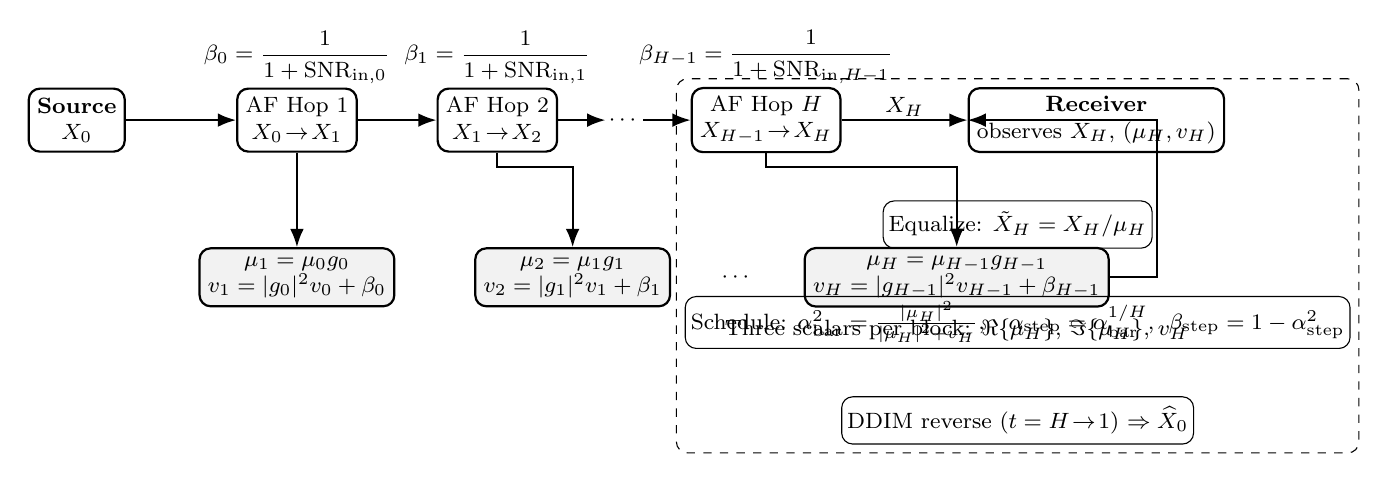
\begin{tikzpicture}[
    >=Latex,
    node distance=8mm and 8mm,
    every node/.style={font=\footnotesize},
    blk/.style={draw, rounded corners, thick, align=center, inner sep=3pt, minimum height=8mm},
    op/.style={draw, rounded corners, thick, align=center, inner sep=3pt, minimum height=6mm, fill=gray!10},
    light/.style={draw, rounded corners, align=center, inner sep=2pt, minimum height=6mm},
    anno/.style={align=left, inner sep=1pt}
]

% Source
\node[blk] (src) {$\mathbf{Source}$\\$X_0$};

% AF hops (compact depiction with ellipsis)
\node[blk, right=14mm of src] (af1) {AF Hop $1$\\$X_0 \!\to\! X_1$};
\node[blk, right=10mm of af1] (af2) {AF Hop $2$\\$X_1 \!\to\! X_2$};
\node[anno, right=6mm of af2] (dots) {$\cdots$};
\node[blk, right=6mm of dots] (afH) {AF Hop $H$\\$X_{H-1} \!\to\! X_H$};

% Sufficient statistics track
\node[op, below=12mm of af1] (stat1) {$\mu_{1}=\mu_0 g_0$\\$v_{1}=|g_0|^2 v_0+\beta_0$};
\node[op, right=10mm of stat1] (stat2) {$\mu_{2}=\mu_1 g_1$\\$v_{2}=|g_1|^2 v_1+\beta_1$};
\node[anno, right=6mm of stat2] (dots2) {$\cdots$};
\node[op, right=6mm of dots2] (statH) {$\mu_{H}=\mu_{H-1} g_{H-1}$\\$v_{H}=|g_{H-1}|^2 v_{H-1}+\beta_{H-1}$};

% Receiver block (dashed fit)
\node[blk, right=16mm of afH] (rx) {$\mathbf{Receiver}$\\observes $X_H$, $(\mu_H,v_H)$};
\node[light, below=6mm of rx, xshift=-10mm] (eq) {Equalize: $\tilde X_H = X_H/\mu_H$};
\node[light, below=6mm of eq] (sched) {Schedule: $\alpha_{\mathrm{bar}}^2=\frac{|\mu_H|^2}{|\mu_H|^2+v_H}$,\quad $\alpha_{\mathrm{step}}=\alpha_{\mathrm{bar}}^{1/H}$,\; $\beta_{\mathrm{step}}=1-\alpha_{\mathrm{step}}^2$};
\node[light, below=6mm of sched] (ddim) {DDIM reverse ($t=H\!\to\!1$) $\Rightarrow \widehat X_0$};

\node[draw, dashed, rounded corners, fit=(rx)(eq)(sched)(ddim), inner sep=3pt] (rxbox) {};

% Arrows along top chain
\draw[->, thick] (src) -- node[above,anno] {} (af1);
\draw[->, thick] (af1) -- (af2);
\draw[->, thick] (af2) -- (dots);
\draw[->, thick] (dots) -- (afH);
\draw[->, thick] (afH) -- node[above,anno] {$X_H$} (rx);

% Arrows for stats
\draw[->, thick] (af1) -- +(0,-0.6) -| (stat1.north);
\draw[->, thick] (af2) -- +(0,-0.6) -| (stat2.north);
\draw[->, thick] (afH) -- +(0,-0.6) -| (statH.north);
\draw[->, thick] (statH.east) -- ++(6mm,0) |- (rx.west);

% Annotations
\node[anno, above=0mm of af1] {$\beta_0=\dfrac{1}{1+\mathrm{SNR}_{\mathrm{in},0}}$};
\node[anno, above=0mm of af2] {$\beta_1=\dfrac{1}{1+\mathrm{SNR}_{\mathrm{in},1}}$};
\node[anno, above=0mm of afH] {$\beta_{H-1}=\dfrac{1}{1+\mathrm{SNR}_{\mathrm{in},H-1}}$};

\node[anno, below=1mm of statH] {Three scalars per block: $\Re\{\mu_H\}$, $\Im\{\mu_H\}$, $v_H$};

\end{tikzpicture}
\caption{AF–DDIM detection pipeline. Each AF hop implements a VP step with $\beta_t=\big(1+\mathrm{SNR}_{\mathrm{in},t}\big)^{-1}$, while relays update the sufficient statistics $(\mu_t, v_t)$. The receiver equalizes by $\mu_H$, constructs a matched VP schedule from $\alpha_{\mathrm{bar}}^2=\frac{|\mu_H|^2}{|\mu_H|^2+v_H}$, and runs a deterministic DDIM reverse to recover $\widehat X_0$.}
\label{fig:af_ddim_pipeline}
\end{figure*}
